\usepackage{comment}
\usepackage{multicol}

\newcommand{\figFOneArch}{
  \begin{figure}[t]
        \begin{center}
        \includegraphics[width=0.7\linewidth]{f1_figures/ag_arch.pdf}
     \caption{Overview of the F1 architecture.}
    \label{fig:f1arch}
  \end{center}
  \end{figure}
}

\newcommand{\figFOneMultDataflow}{
  \begin{figure}[t]
        \begin{center}
     \includegraphics[width=0.7\columnwidth]{f1_figures/ag_mult_dataflow.pdf}
    \caption{Example matrix-vector multiply using FHE.}
    \label{fig:f1MultDataflow}
    \end{center}
  \end{figure}
}

\newcommand{\figFOneOpBreakdown}{
    \begin{figure}[t]
    \begin{center}
        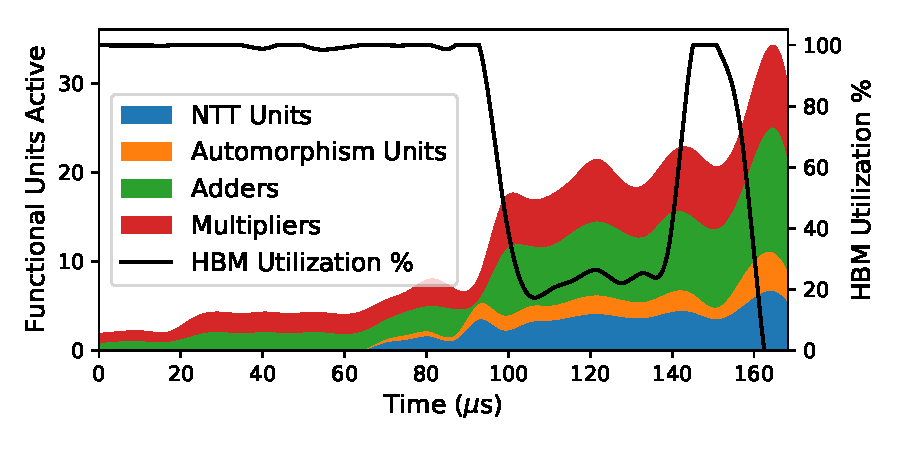
\includegraphics[width=0.65\columnwidth]{f1_plots/lolaptwTimeplot.pdf}
        \caption{Functional unit and HBM utilization over time for the LoLa-MNIST PTW benchmark.}
        \label{fig:f1opBreakdown}
    \end{center}
    \end{figure}
}

\newcommand{\figFOneCompilerOverview}{
  \begin{figure}[t]
        \begin{center}
     \includegraphics[width=0.65\columnwidth]{f1_figures/ag_compiler_overview.pdf}
    \caption{Overview of the F1 compiler.}
    \label{fig:f1compilerOverview}
    \end{center}
  \end{figure}
}

\newcommand{\figFOneautfu}{
\setlength{\columnsep}{7pt}
  \begin{wrapfigure}{r}{0.3\linewidth}
     \includegraphics[width=0.25\columnwidth]{f1_figures/ag_aut_fu.pdf}
    \caption{Automorphism unit.}
    \label{fig:f1aut_fu}
  \end{wrapfigure}
}

\newcommand{\figFOneAutomorphism}{
  \begin{figure}[t]
        \begin{center}
    \includegraphics[width=0.1\columnwidth]{f1_figures/ag_automorphism.pdf}
    \caption{Applying $\sigma_3$ on an RNS polynomial of four 4-element chunks by using only permutations local to chunks.}
    \label{fig:f1automorphism}
    \end{center}
  \end{figure}
}

\newcommand{\figFOneTranspose}{
  \begin{figure}[t]
    \centering
    \includegraphics[width=0.5\columnwidth]{f1_figures/ag_transpose.pdf}
    \caption{The transpose unit.}
    \label{fig:f1transpose}
  \end{figure}
}

\newcommand{\figFOneFourStepNTT}{
  \begin{figure}[t]
    \begin{center}
    \includegraphics[width=0.8\columnwidth]{f1_figures/ag_four_step_ntt.pdf}
    \caption{Example of a four-step NTT datapath that uses 4-point NTTs to implement 16-point NTTs.}
    \label{fig:f1fourStepNTT}
    \end{center}
  \end{figure}
}

\newcommand{\figFOneQuadrantSwap}{
  \begin{figure}[t]
    \centering
    \includegraphics[width=0.8\columnwidth]{f1_figures/ag_quadrant_swap.pdf}
    \caption{Transpose unit (right) and its component quadrant-swap unit (left).}
    \label{fig:f1quadrantSwap}
  \end{figure}
}

\newcommand{\figFOneOverview}{
  \begin{figure}[h] % dsm: acmart crap bleeds onto the second column, makes it hard for this figure to be on top, so make it [h]
    \centering
    \includegraphics[width=\columnwidth]{f1_figures/ag_overview.pdf}
    \caption{FHE allows a user to securely offload computation to an untrusted server.}
    %old: \caption{Workflow showing how FHE is used to securely offload computation to an untrusted server.}
    \label{fig:f1overview}
  \end{figure}
}

\newcommand{\figFOneFUSweep}{
  \begin{figure}[t]
        \begin{center}
     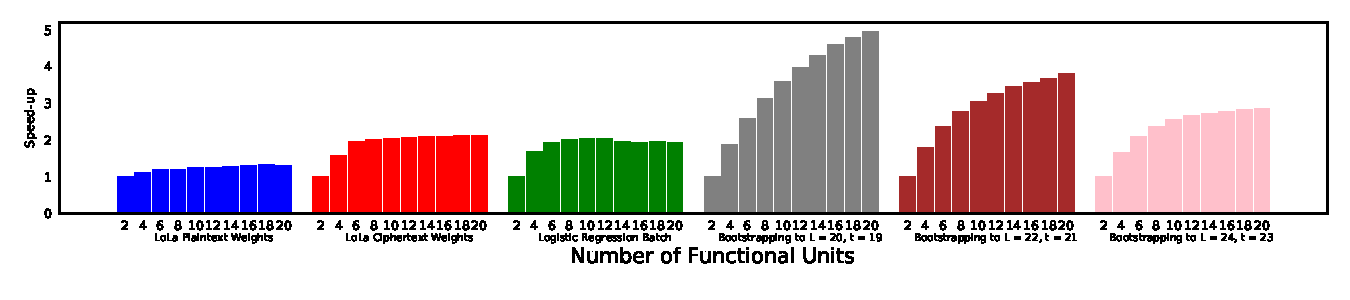
\includegraphics[width=\columnwidth]{f1_plots_unused/sweepFUs.pdf}
    \caption{Performance of our benchmarks with varying number of functional unit clusters.}
    \label{fig:f1sweepFUs}
    \end{center}
  \end{figure}
}

\newcommand{\figFOneBWSweep}{
  \begin{figure}[t]
        \begin{center}
     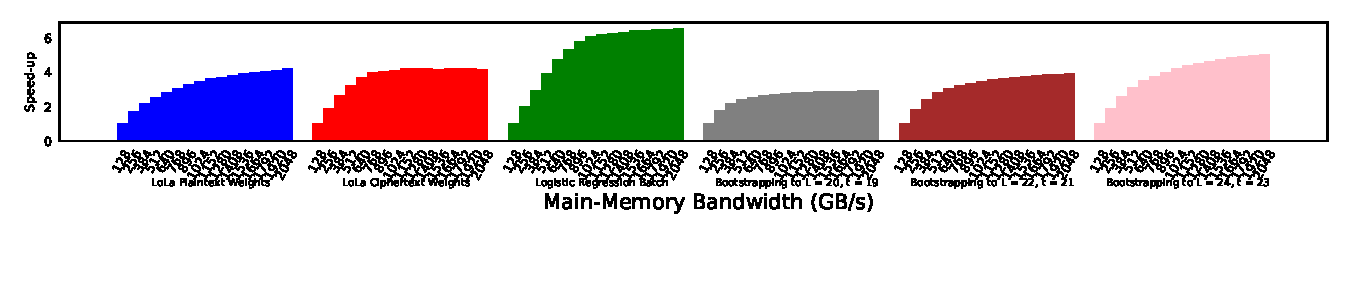
\includegraphics[width=\columnwidth]{f1_plots_unused/sweepBW.pdf}
    \caption{Performance of our benchmarks across various main memory bandwidths.}
    \label{fig:f1sweepBW}
    \end{center}
  \end{figure}
}

\newcommand{\figFOneDataMovement}{
\begin{figure}
  \centering
  \captionsetup[subfigure]{labelformat=empty}
  \begin{subfigure}[b]{0.4\columnwidth}
    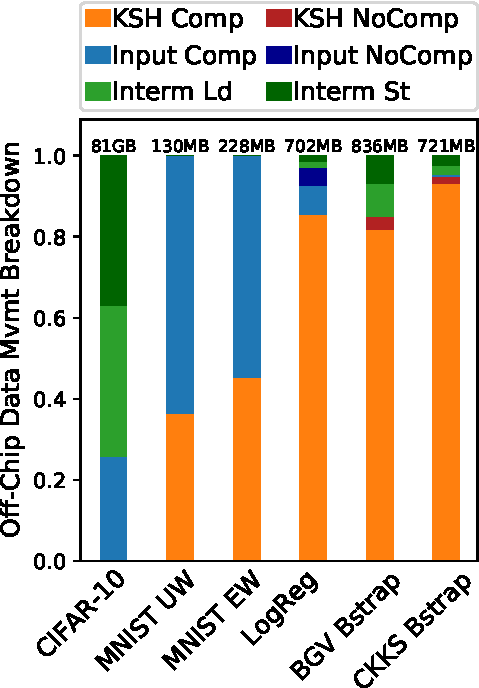
\includegraphics[width=\linewidth]{f1_plots/dataMovement.pdf}
    \caption{}
    \label{fig:f1dataMovement}
  \end{subfigure}
  \hfill %%
  \begin{subfigure}[b]{0.4\columnwidth}
    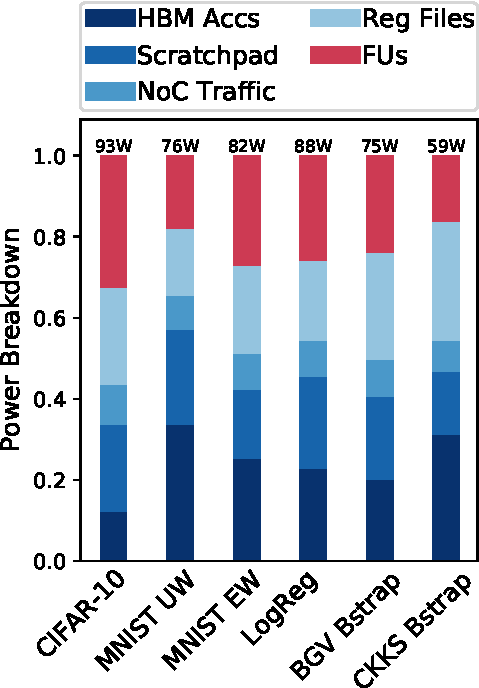
\includegraphics[width=\linewidth]{f1_plots/power.pdf}
    \caption{}
    \label{fig:f1power}
  \end{subfigure}
  \begin{center}
    (a) \hspace{0.6\columnwidth} (b)
  \end{center}
  \caption{Per-benchmark breakdowns of (a) data movement and (b) average power for F1.}
\end{figure}
}

\newcommand{\figFOneConfigs}{
  \begin{figure}[t]
    \begin{center}
     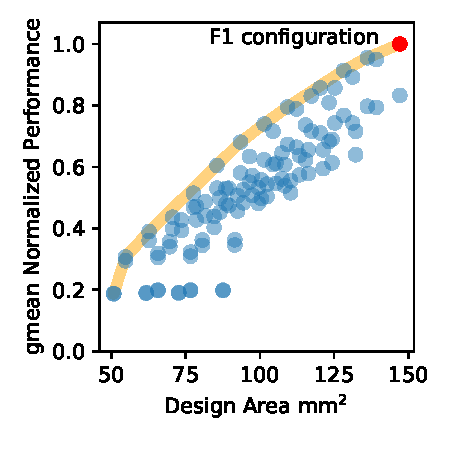
\includegraphics[width=0.35\columnwidth]{f1_plots/configs.pdf}
    \caption{Performance vs. area across F1 configurations.}
    \label{fig:f1pareto}
    \end{center}
  \end{figure}
}

\newcommand{\figFOneScratchpadSweep}{
  \begin{figure}[t]
        \begin{center}
     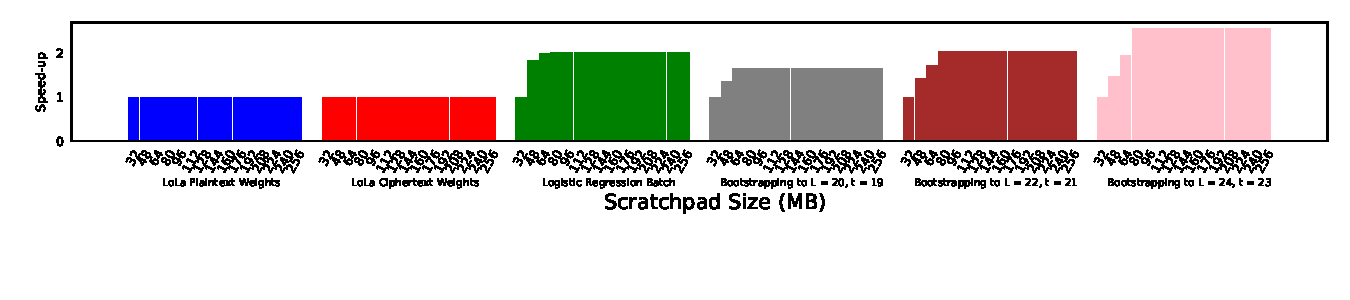
\includegraphics[width=\columnwidth]{f1_plots_unused/sweepScratchpad.pdf}
    \caption{Performance of our benchmarks across various scratchpad sizes.}
    \label{fig:f1sweepScratchpad}
    \end{center}
  \end{figure}
}

\newcommand{\tblFOneGF}{
  \begin{table}[t]
    \begin{center}
      \begin{normalsize}
        \begin{tabular}{lrrr}
          \toprule
          Component & Area [mm$^2$] & TDP [W] \\
          \midrule
          NTT FU & 2.27 & 4.80  \\
          Automorphism FU & 0.58 & 0.99  \\
          %Transpose & 0.28 & \tmp{???} & - \\
          Multiply FU & 0.25 & 0.60  \\
          Add FU & 0.03 & 0.05  \\
          Vector RegFile (512\,KB) & 0.56 & 1.67 \\
          \textbf{Compute cluster} & 3.97 & 8.75 \\
          (NTT, Aut, 2$\times$ Mul, 2$\times$ Add, RF) & & \\
          \textbf{Total compute} (16 clusters) &  \textbf{63.52} & \textbf{140.0} \\
          \midrule
          Scratchpad (16$\times$4\,MB banks) & 48.09 & 20.35 \\
          3$\times$NoC (16$\times$16 512\,B bit-sliced~\cite{passas:tocaid12:crossbar}) & 10.02 & 19.65 \\
          Memory interface (2$\times$HBM2 PHYs) & 29.80 & 0.45 \\
          \textbf{Total memory system} &  \textbf{87.91} & \textbf{40.45} \\
          \midrule
          \textbf{Total F1} &  \textbf{151.4} & \textbf{180.4} \\
          \bottomrule
        \end{tabular}
      \end{normalsize}
    \end{center}
    \caption{Area and Thermal Design Power (TDP) of F1, and breakdown by component.}
    \label{tbl:f1GF12}
  \end{table}
}


\newcommand{\tblFOneNomenclature}{
   \begin{table}[t]
     \begin{normalsize}
        \begin{center}
           \begin{tabular}{ll}
              \toprule
              \textbf{Param} & \textbf{Definition} \\
              \midrule
               \multicolumn{2}{c}{FHE Parameters} \\
              \midrule
              $N$ & Number of vector elements / polynomial coefficients \\
              $Q$ & Ciphertext modulus \\
              $t$ & Plaintext modulus \\
              \midrule
               \multicolumn{2}{c}{Architecture Parameters} \\
              \midrule
              $L$ & Number of RNS polynomials per ciphertext polynomial \\
              $q_i$ & The $i$-th RNS modulus ($Q = q_0q_1...q_{L-1}$) \\
              $E$ & Number of vector lanes \\
              $V$ & Vector operation initiation interval ($V = N/E$) \\ % dsm: Chimes? I don't know of a good nomenclature for this...
              \bottomrule
           \end{tabular}
           \label{tbl:f1nomenclature}
        \end{center}
        \caption{Nomenclature of key parameters in this paper.}
     \end{normalsize}
   \end{table}
}

\newcommand{\tblFOneModMult}{
  \begin{table}[t]
    \begin{normalsize}
      \begin{center}
        \begin{tabular}{lrrr}
          \toprule
          Multiplier & Area [$\mu$m$^2$] & Power [mW] & Delay [ps] \\
          \midrule
          Barrett & $5,271$ & $18.40$ & 1,317 \\
          Montgomery & $2,916$ & $9.29$ & 1,040 \\
          NTT-friendly & $2,165$ & $5.36$ & 1,000 \\ % assumes q = 2^11m+1
          \midrule
          \textbf{FHE-friendly (ours)} & $1,817$ & $4.10$ & 1,000 \\
          \bottomrule
        \end{tabular}
        \caption{Area, power, and delay of modular multipliers.}
        \label{tbl:f1modMult}
      \end{center}
    \end{normalsize}
  \end{table}
}


\newcommand{\tblFOneMicrobenchmark}{
  \begin{table*}[b]
    \begin{scriptsize}
      \begin{center}
%\resizebox{\linewidth}{!}{
      \begin{tabular}{l|rrr|rrr|rrr}
        \toprule
        & \multicolumn{3}{c|}{$N = 2^{12}$, $\log Q = 109$} &
        \multicolumn{3}{c|}{$N = 2^{13}$, $\log Q = 218$} &
        \multicolumn{3}{c}{$N = 2^{14}$, $\log Q = 438$} \\

        & \textbf{F1} & vs.\ CPU & vs.\ HEAX$_\sigma$ & \textbf{F1} & vs.\ CPU & vs.\ HEAX$_\sigma$ & \textbf{F1} & vs.\ CPU & vs.\ HEAX$_\sigma$\\

        \midrule

        % --- NTT

        % N=2**12, logQ = 109
        NTT
        &\textbf{12.8} % our
        &17,148$\times$ % CPU
        &1,600$\times$ % HEAX

        % N=2**13, logQ = 218
        &\textbf{44.8} % our
        &10,736$\times$ % CPU
        &1,733$\times$ % HEAX

        % N=2**14, logQ = 438
        &\textbf{179.2} % our
        &8,838$\times$ % CPU
        &1,866$\times$ % HEAX
        \\
        % --- Automorph. w/out k-s

        % N=2**12, logQ = 109
        Automorphism
        &\textbf{12.8} % our
        &7,364$\times$ % CPU
        &440$\times$ % HEAX

        % N=2**13, logQ = 218
        &\textbf{44.8} % our
        &8,250$\times$ % CPU
        &426$\times$ % HEAX

        % N=2**14, logQ = 438
        &\textbf{179.2} % our
        &16,957$\times$ % CPU
        &430$\times$ % HEAX
        \\

        \midrule

        % --- Ctxt-Ctxt Mult.

        % N=2**12, logQ = 109
        Hom. mult.
        &\textbf{60.0} % our - % 60 MULS * 32 * 1/(32) = 60 cycles
        &48,640$\times$ % CPU
        &172$\times$ % HEAX

        % N=2**13, logQ = 218
        &\textbf{300} % our
        &27,069$\times$ % CPU
        &148$\times$ % HEAX

        % N=2**14, logQ = 438
        &\textbf{2,000} % our
        &14,396$\times$ % CPU
        &190$\times$ % HEAX
        \\

        % --- Automorph. w/ k-s

        % N=2**12, logQ = 109
        Hom. rot.
        &\textbf{40.0} % our
        &17,488$\times$ % CPU
        &256$\times$ % HEAX

        % N=2**13, logQ = 218
        &\textbf{224} % our
        &10,814$\times$ % CPU
        &198$\times$ % HEAX

        % N=2**14, logQ = 438
        &\textbf{1,680} % our
        &6,421$\times$ % CPU
        &227$\times$ % HEAX
        \\

        \bottomrule
      \end{tabular}
      %}
      \end{center}
      \caption{Performance on microbenchmarks: F1's \textbf{reciprocal throughput, in nanoseconds per ciphertext operation} (lower is better) and speedups over CPU and HEAX$_\sigma$ (HEAX augmented with scalar automorphism units) (higher is better).}
      \label{tbl:f1microbenchmark}
    \end{scriptsize}
  \end{table*}
    % dsm: Now explained in text
    %\footnotetext[2]{We assume an SRAM array is used to perform an automorphism via random reads because HEAX does not report how they implement automorphisms.}
    %     \footnotetext[3]{We assume throughput is bottleneck on either the automorphism or keyswitching throughput, whichever is smaller.}
}


\newcommand{\tblFOneBenchmark}{
  \begin{table}[t]
    \begin{normalsize}
      \begin{center}
      \begin{tabular}{lrrr}
        \toprule
        Execution time (ms) on & CPU & F1 & Speedup \\

        \midrule
        LoLa-CIFAR Unencryp. Wghts. & $1.2\times10^6$ & \textbf{241} & $5,011$\x \\
        LoLa-MNIST Unencryp. Wghts. & $2,960$ & \textbf{0.17} & $17,412$\x \\
        LoLa-MNIST Encryp. Wghts. & $5,431$ & \textbf{0.36} & $15,086$\x \\
        Logistic Regression & $8,300$ & \textbf{1.15} & $7,217$\x \\
        DB Lookup & $29,300$ & \textbf{4.36} & $6,722$\x \\
        BGV Bootstrapping & $4,390$ & \textbf{2.40} & $1,830$\x \\  % L=24
        CKKS Bootstrapping & $1,554$ & \textbf{1.30} & $1,195$\x \\    % L=24
        \midrule

        \textbf{gmean speedup} &&& $5,432$\x \\
        % CKKS Bootstrapping $L=22$ & $1456$ & \textbf{2.2} & $662$\x \\
        % CKKS Bootstrapping $L=20$ & $1314$ & \textbf{1.9} & $692$\x \\
        \bottomrule
      \end{tabular}
   \end{center}
      \hfill\footnotemark[1]{LoLa's release did not include MNIST with encrypted weights, so we reimplemented it in HELib.}\quad\mbox{}
    \end{normalsize}
      \caption{Performance of F1 and CPU on full FHE benchmarks: execution times in milliseconds
      and F1's speedup.}      
      \label{tbl:f1benchmark}
  \end{table}
}

\newcommand{\tblFOnePrimitiveOps}{
  \begin{table}[t]
    \begin{normalsize}
      \begin{center}
        \caption{Operations in BGV \cite{}, CKKS \cite{}, and GSW \cite{} schemes and their constituent
        \textit{primitive operations}, which F1 FUs acelerate. BGV and CKKS use very similar FHE operations
        and differ mainly in encryption/decryption.}
        \begin{tabular}{l|rr}
          \toprule
          & \multicolumn{2}{c}{\textbf{Required primitive operations}} \\
          \textbf{Operation} & \textbf{BGV/CKKS} & \textbf{GSW} \\
          \midrule
          Ciphertext add & add & add \\
          Ciphertext mult & NTT, mult & NTT, mult, add \\
          Key switching/relin & NTT, mult, add & N/A \\
          Mod switching & NTT, reduce, add & NTT, reduce, add \\
          Bootstrapping & automorphism, all ops & automorphism, all ops \\
          \bottomrule
        \end{tabular}
        \label{tbl:f1primitiveOps}
      \end{center}
    \end{normalsize}
  \end{table}
}

\newcommand{\cipher}{\textsf{Ciphertext}}
\newcommand{\plain}{\textsf{Plaintext Vector}}
\newcommand{\scalar}{\textsf{Plaintext Scalar}}

\newcommand{\tblFOneDSLOps}{
  \begin{table}[t]
    \begin{normalsize}
      \begin{center}
        \caption{Supported FHE Operations and Types}
        \begin{tabular}{l|r}
            \textbf{Operation} & \textbf{Type}\\
            \midrule
            \textsf{Mul} & $\cipher \times \cipher \rightarrow \cipher$ \\
            \textsf{MulPlaintext} & $\cipher \times \plain \rightarrow \cipher$ \\
            \textsf{MulScalar} & $\cipher \times \scalar \rightarrow \cipher$ \\
            \textsf{Add} & $\cipher \times \cipher \rightarrow \cipher$ \\
            \textsf{AddPlaintext} & $\cipher \times \plain \rightarrow \cipher$ \\
            \textsf{AddScalar} & $\cipher \times \scalar \rightarrow \cipher$ \\
            \textsf{Rotate} & $\cipher \times \scalar \rightarrow \cipher$ \\
            \textsf{ModDown} & $\cipher \times \scalar \rightarrow \cipher$ \\
        \end{tabular}
      \end{center}
    \end{normalsize}
  \end{table}
}


\newcommand{\tblFOneSensitivity}{
  \begin{table}[t]
    \begin{normalsize}
      \begin{center}
        \begin{tabular}{lrrr}
            \toprule
            Benchmark & LT NTT & LT Aut & CSR \\
            \midrule
            LoLa-CIFAR Unencryp. Wghts. & 3.5\x & 12.1\x & ---\footnotemark[1] \\
            LoLa-MNIST Unencryp. Wghts. & 5.0\x & 4.2\x & 1.1\x \\
            LoLa-MNIST Encryp. Wghts. & 5.1\x & 11.9\x & 7.5\x \\
            Logistic Regression & 1.7\x & 2.3\x & 11.7\x \\
            DB Lookup & 2.8\x & 2.2\x & ---\footnotemark[1] \\
            BGV Bootstrapping & 1.5\x & 1.3\x & 5.0\x \\
            CKKS Bootstrapping & 1.1\x & 1.2\x & 2.7\x \\
            \midrule
            \textbf{gmean speedup} & 2.5\x & 3.6\x & 4.2\x \\
            \bottomrule
        \end{tabular}
      \end{center}
      \hfill\footnotemark[1]{CSR is intractable for this benchmark.}\quad\mbox{}
    \end{normalsize}
        \caption{Speedups of F1 over alternate configurations: %without our contributions:
          LT NTT/Aut = Low-throughput NTT/Automorphism FUs; CSR = Code Scheduling to minimize Register Usage~\cite{goodman:ics1988:code}.}
        \label{tbl:f1sensitivity}
  \end{table}
}

\providecommand{\C}{\textsf{Scalar}}
\newcommand{\V}{\textsf{Vector}}
\newcommand{\q}{\textsf{Modulus}}

\newcommand{\tblFOneISA}{
  \begin{table}[t]
  \begin{normalsize}
  \begin{center}
  \caption{F1 ISA}
  \begin{tabular}{lr}
  \toprule
  Instruction & Type \\
  \midrule
  \texttt{ADD} & $\V \times \V \times \q \rightarrow \V$ \\
  \texttt{ADD\_SCALAR} & $\V \times \C \times \q \rightarrow \V$ \\
  \texttt{MUL} & $\V \times \V \times \q \rightarrow \V$ \\
  \texttt{MUL\_SCALAR} & $\V \times \C \times \q \rightarrow \V$ \\
  \texttt{NTT} & $\V \times \q \rightarrow \V$ \\
  \texttt{INTT} & $\V \times \q \rightarrow \V$ \\
  \texttt{AUTOMORPHISM} & $\V \times \C \rightarrow \V$ \\
  \end{tabular}
  \label{tbl:f1isa}
  \end{center}
  \end{normalsize}
  \end{table}
}

